\documentclass[11pt]{article}

\usepackage{pdflscape}
\usepackage{graphicx}
\usepackage[hidelinks]{hyperref}

\begin{document}

\begin{titlepage}
	\begin{center}
		
		\begin{figure}[t]
			\centering
			
\includegraphics[width=350px]{../Images/UP_Logo.png}
		\end{figure}
		
		% Title
		\textsc{\large } \\ 
		\vspace{2cm}
		\textbf{\Huge IMY 310 Project  \\
			Project Plan \\
			(Phase 1)} \\ 

		\textsc{\large } \\ 
		\vspace{0.75cm}

		\textbf{\Large AgriSales Magazine} \\ 
		
		\begin{flushright} \large
			Azhar Mohungoo \emph{12239799} \newline
			Daniel Malangu \emph{} \newline
			Kudzai  	\emph{} \newline
			\newline
			Group Name  \emph{} \newline
			\end{flushright}
		%\end{minipage}
		
	\end{center}
\end{titlepage}


\tableofcontents

\newpage

\section{Major Sections}
	\subsection{Homepage}
		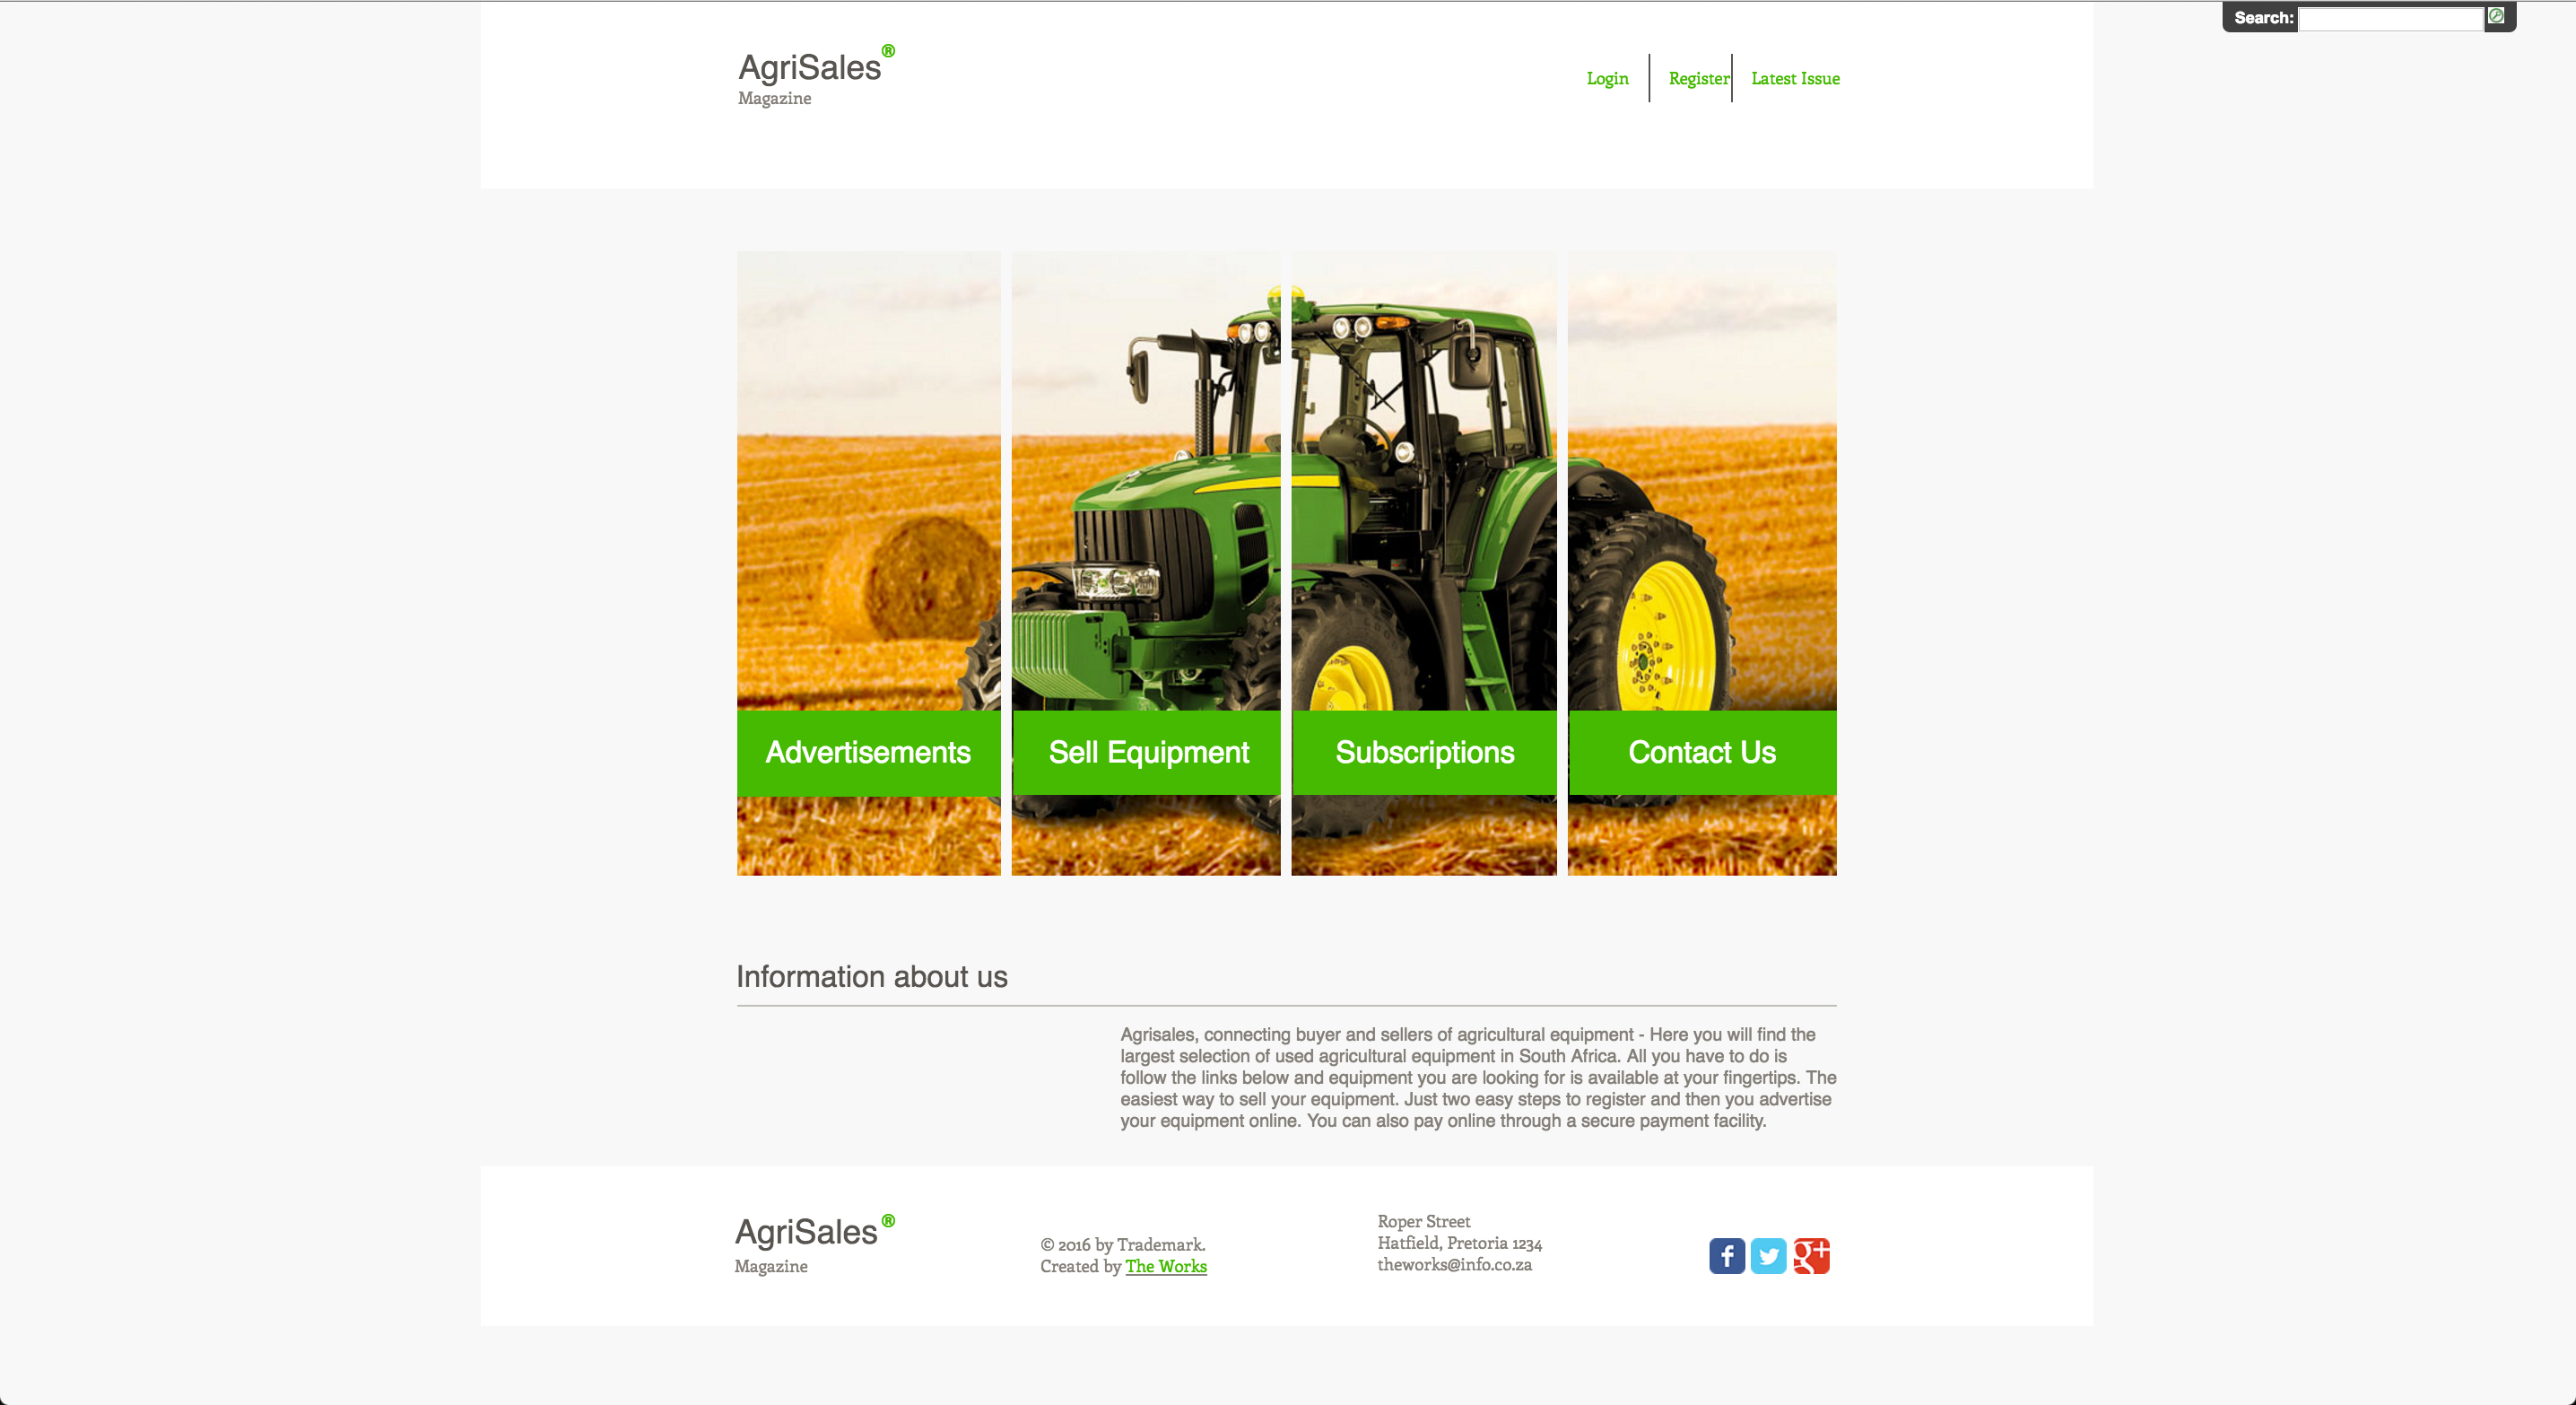
\includegraphics[width=\textwidth]{../Images/Pages/Homepage} \\
		
		**NOTE** From this point onwards, we will only be displaying the content of the body of the HTML pages as the format of the pages, i.e. the header and footer, stay consistent throughout the website.
		
	\subsection{Login}
	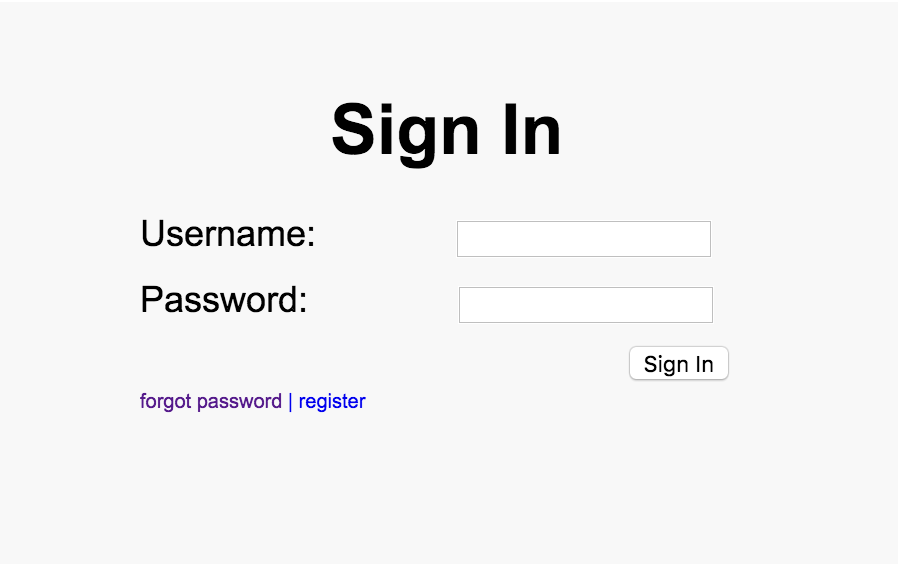
\includegraphics[width=0.75\textwidth]{../Images/Pages/Login}
	\subsection{Register}
		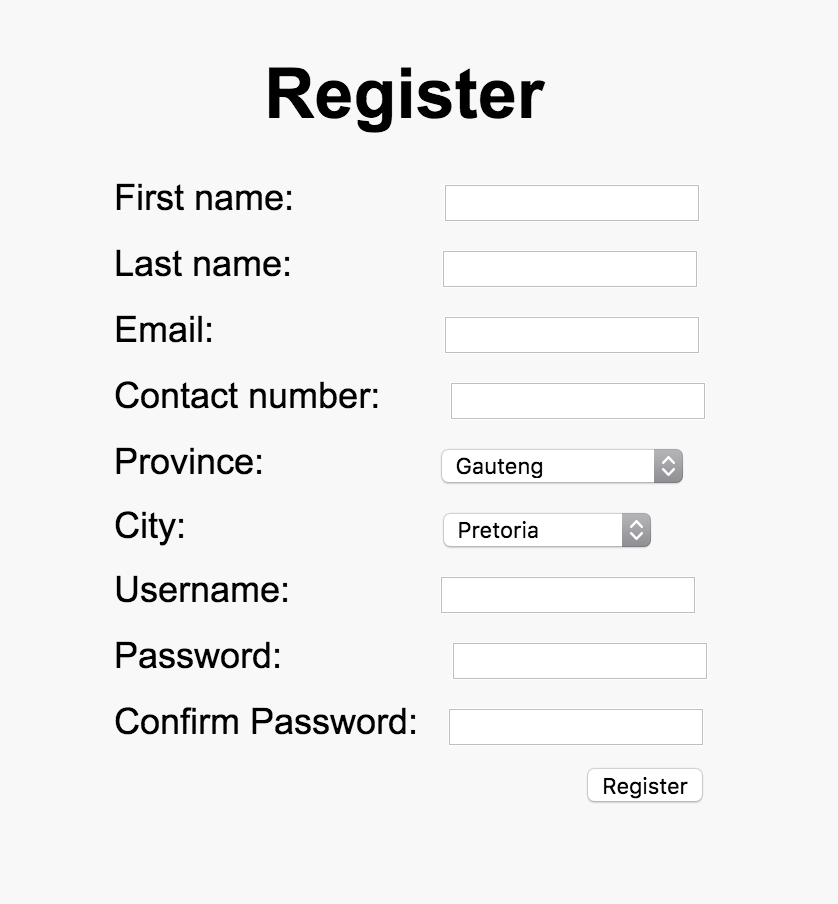
\includegraphics[width=0.55\textwidth]{../Images/Pages/Register}
	\subsection{Advertisements}
	\subsection{Sell Equipment}
	\subsection{Subscriptions}
	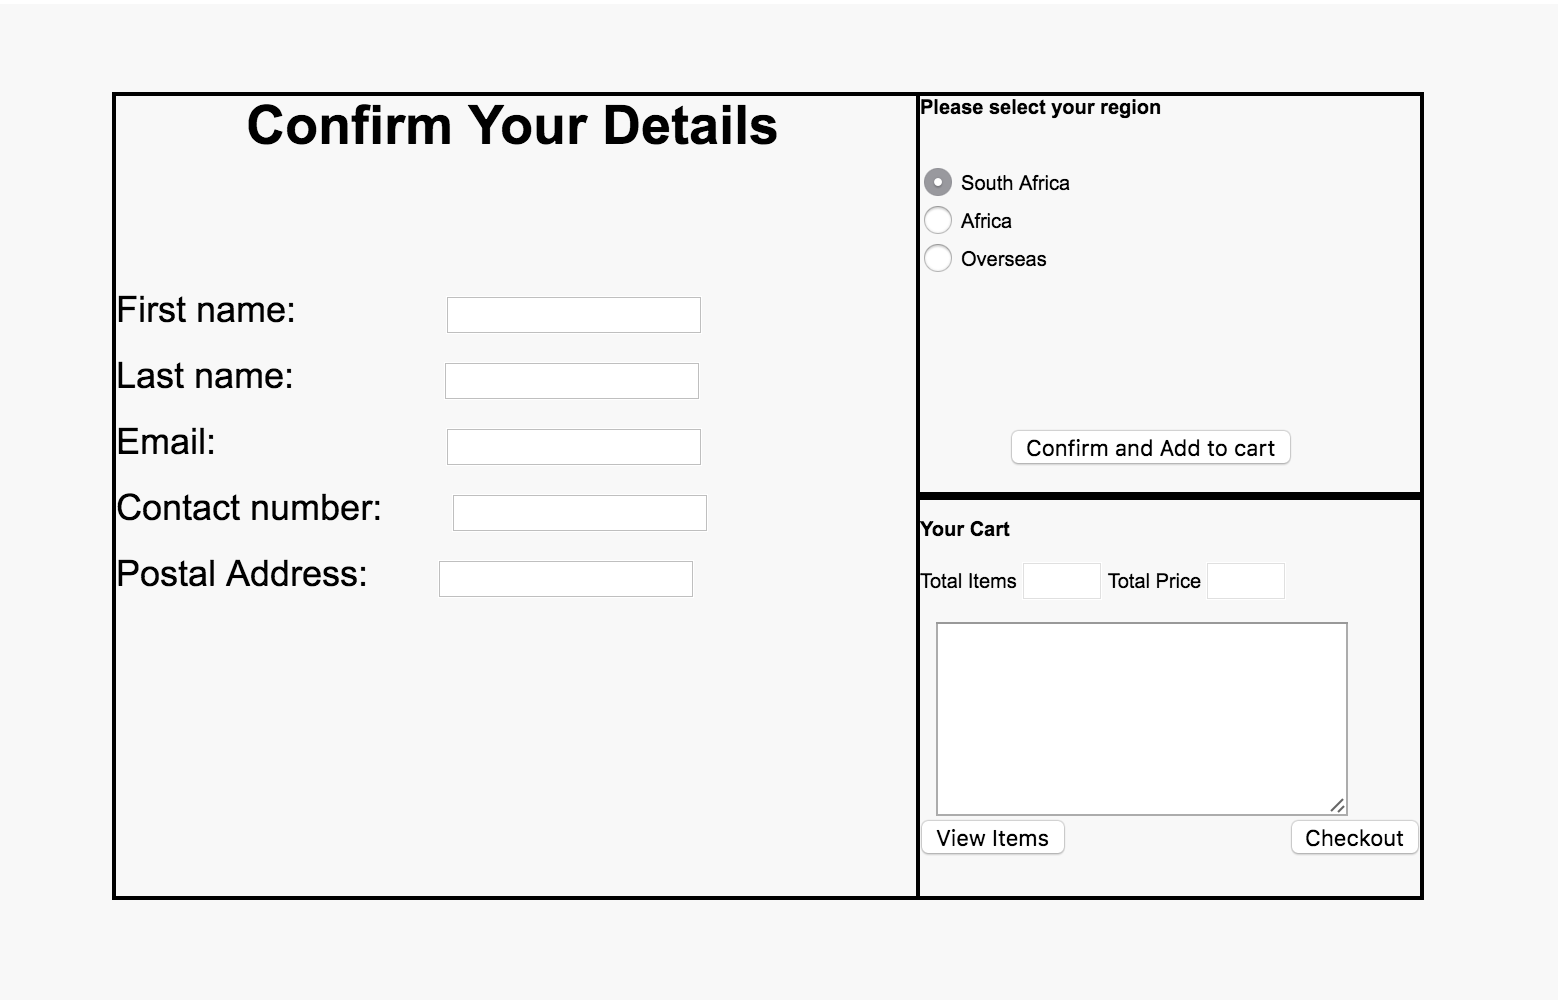
\includegraphics[width=\textwidth]{../Images/Pages/Subscriptions}
	\subsection{Contact Us}
		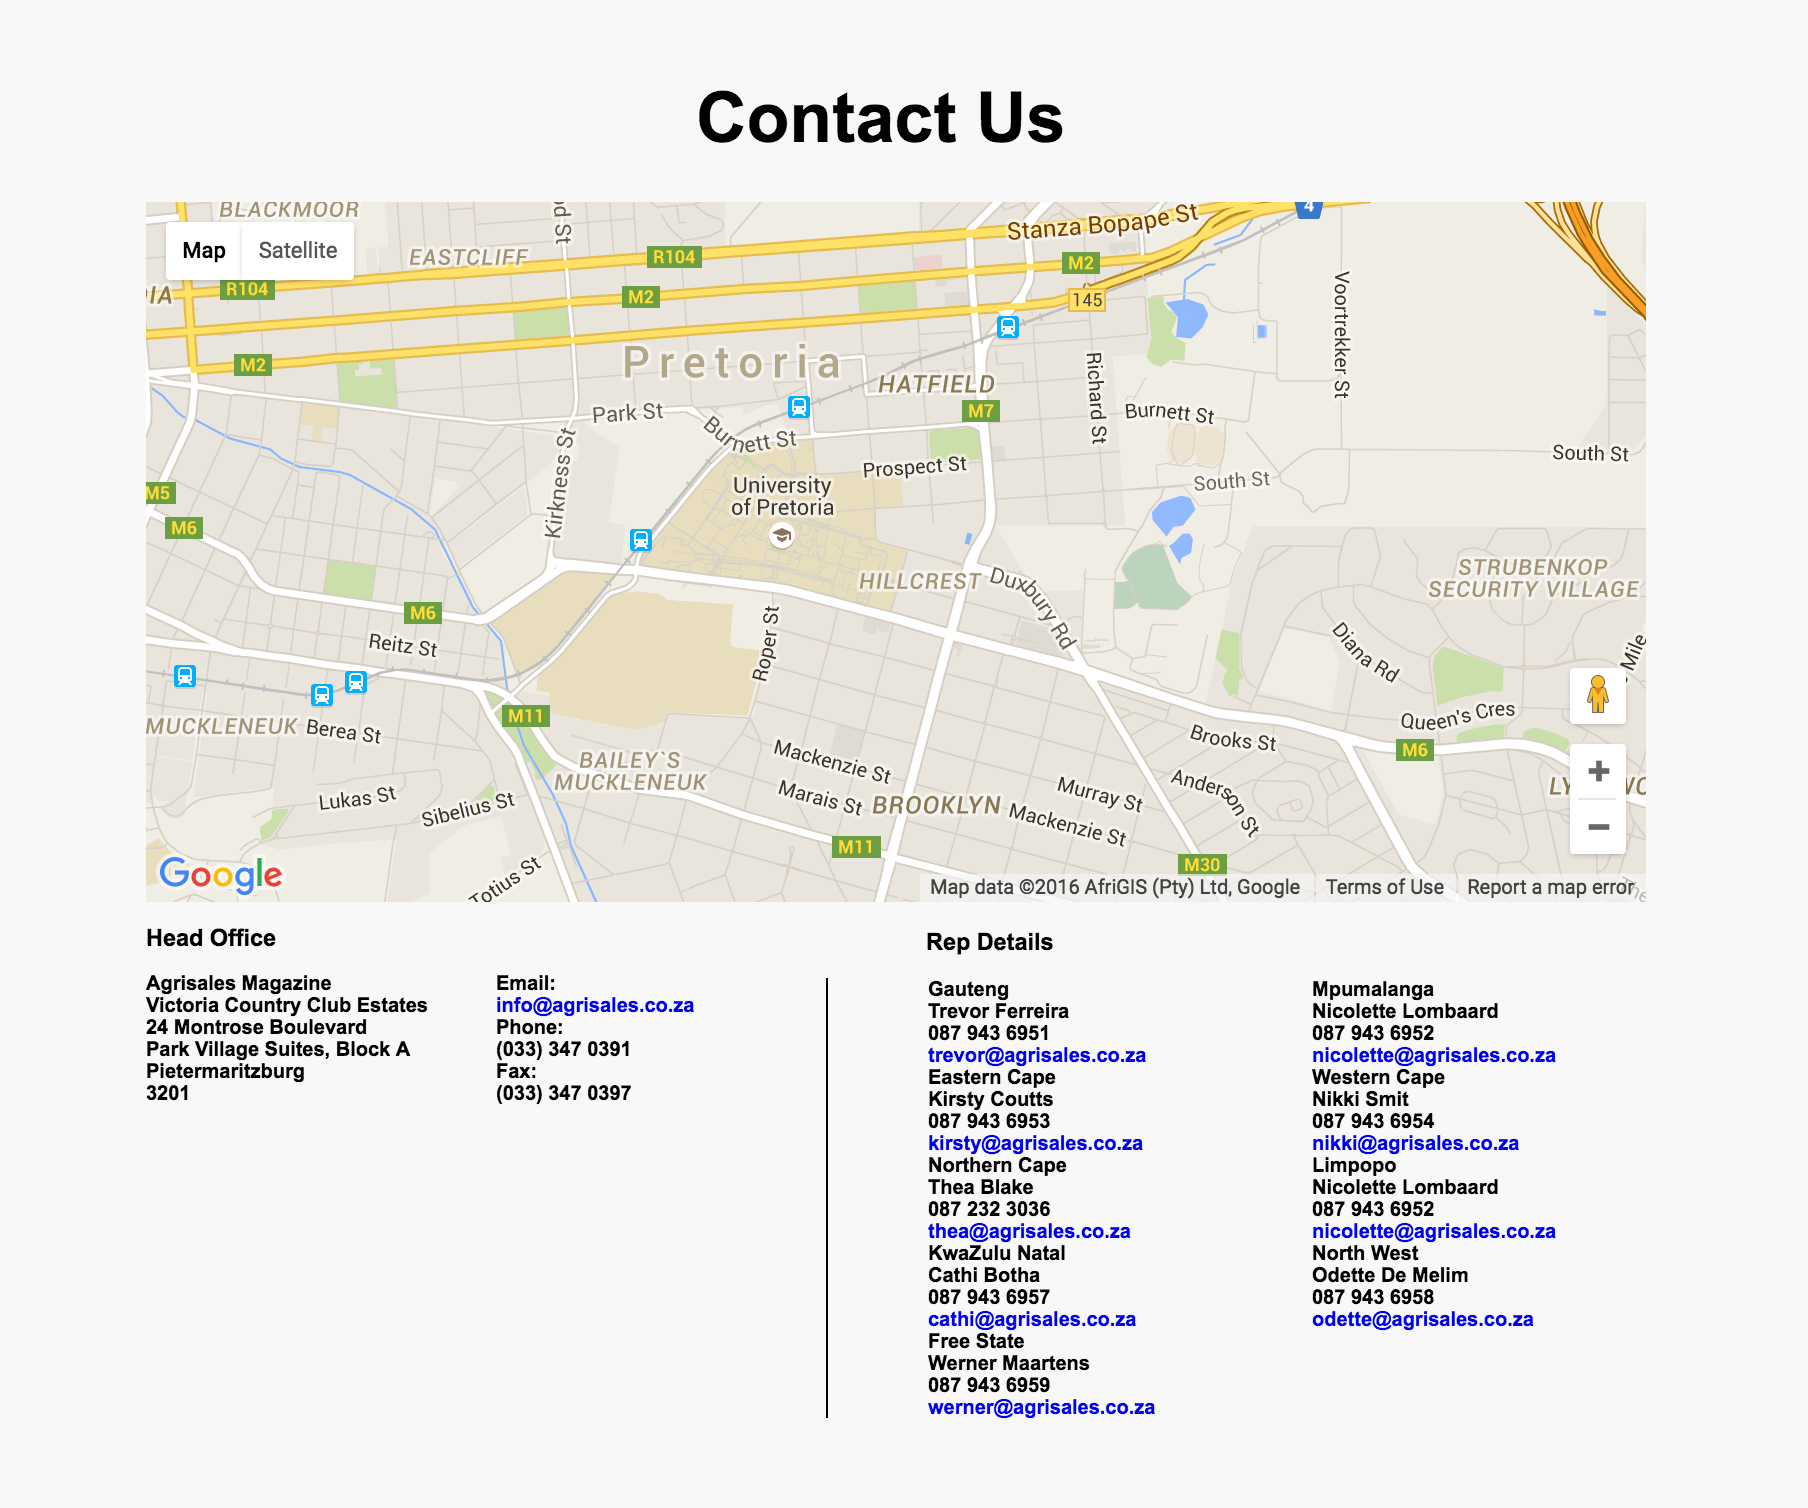
\includegraphics[width=\textwidth]{../Images/Pages/ContactUs}

\newpage

\section{Tasks}
	\begin{enumerate}
		\item Where is the location (city) of the AgriSales head office?
				\begin{enumerate}
					\item Before: Homepage.html \\ \\
						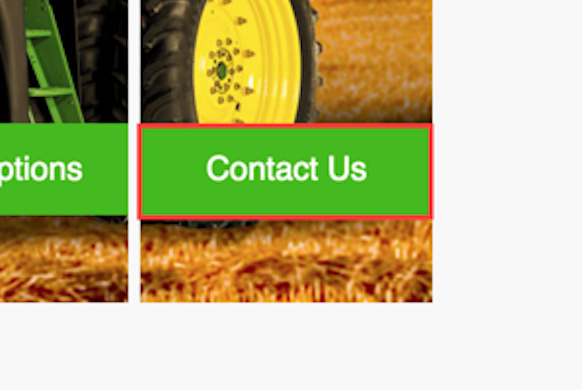
\includegraphics[width=0.5\linewidth]{../Images/Tasks/Task1Before}
					\item After: ContactUs.html \\ \\
						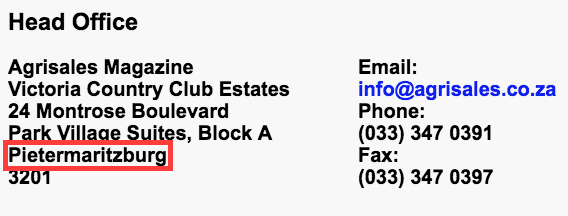
\includegraphics[width=0.5\linewidth]{../Images/Tasks/Task1After}
				\end{enumerate}
		\item Download the latest issue of the magazine.
		\item Register yourself a new AgriSales account.
		\item Search for the contact details of the owner of blue tractor made in 2003.
		\item 
		\item 
		\item 
		\item 
		\item 
		\item 
	\end{enumerate}

\end{document}
